% !TeX root = main.tex
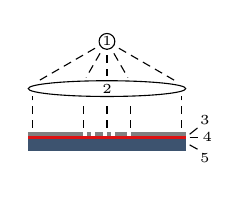
\begin{tikzpicture}
    % Sample
    \fill[fill={rgb:red,66;green,91;blue,121}] (-1,-1.24) rectangle (1,-1.39);
    \draw (1.05,-1.315) to node [below right = -.4 mm] {\tiny $5$} (1.15,-1.37);
    % Resist
    \fill[fill={rgb:red,198;green,15;blue,15}] (-1,-1.20) rectangle (1,-1.24);
    \draw (1.05,-1.22) to node [right = -.1 mm] {\tiny $4$} (1.15,-1.22);
    % Mask
    \foreach \x/\y in {0/.7,.75/.8,.85/0.95,1/1.05,1.1/1.25,1.3/2}
        \fill[fill=gray] (\x-1,-1.15) rectangle (\y-1,-1.20);
    \draw (1.05,-1.18) to node [above right = -.4 mm] {\tiny $3$} (1.15,-1.10);
    % Lens
    \draw (0,-.6) ellipse [x radius=1, y radius=.1] node {\tiny $2$};
    % Light source
    \foreach \angle/\r in {210/1,240/.53,270/.44,300/.53,330/1}
        \draw[densely dashed] (0,0) -- (\angle:\r);
    \foreach \x/\y in {-.95/.7,-.3/.75,0/.75,.3/.75,.95/.7}
        \draw[densely dashed] (\x,-1.1) -- (\x,-\y);
    \draw[fill=white] (0,0) ellipse [x radius=.1, y radius=.1] node {\tiny $1$};
\end{tikzpicture}
